\chapter{Sistemas de Dinámica Compleja}
\label{capSist}

En los últimos años se ha establecido que existen sistemas deterministas que rompen con el preconcepto de que los sistemas físicos pueden clasificarse en dos conjuntos disjuntos: sistemas deterministas y sistemas estocásticos.
El concepto antiguo era que un sistema determinista es aquél para el cual conocemos el modelo y por lo tanto es posible predecir con exactitud la evolución de sus variables de estado.
Se utilizan en su descripción ecuaciones diferenciales o de recurrencia.
Por otra parte un sistema estocástico es aquél para el cual el modelo no se conoce o se lo supone sumamente complejo como para ser obtenido, de modo que se adopta la estrategia de estudiar sus variables de estado en forma estadística.
Se utilizan entonces en la descripción ecuaciones diferenciales o de recurrencia estocásticas.

El caos determinista demostró que complejidad en la evolución temporal no es sinónimo de complejidad en el modelo, cuando hay alinealidad: modelos deterministas muy simples originan señales de aspecto estocástico.
La sensibilidad a las condiciones iniciales hace que en estos sistemas la predictibilidad sea a corto plazo (luego de un tiempo finito es imposible predecir la evolución) lo que ubica a estos sistemas en una posición intermedia entre determinista y estocástico \cite{Liao2013a}.

Como consecuencia se desarrollaron en los últimos años un número creciente de aplicaciones de los sistemas caóticos, empleándolos principalmente como generadores de ruido controlado \cite{DeMicco2007C}, generadores de números pseudoaleatorios \cite{DeMicco2007A}, portadoras de señales \cite{DeMicco2007B}, sistemas de encriptado \cite{Machado2004, Smaoui2009}, etc.

Hoy en día, los sistemas dinámicos son un objeto de estudio interdisciplinario, aunque originalmente fue una rama de la física.
Todo comenzó a mediados del 1600, cuando Newton inventó las ecuaciones diferenciales, descubriendo sus leyes del movimiento de gravitación universal, y las combinó con las leyes de Kepler sobre el movimiento planetario.
Específicamente, Newton resolvió el problema de los dos cuerpos (por ejemplo el sistema tierra-sol).

Subsecuentes generaciones de matemáticos y físicos intentaron extender los métodos analíticos de Newton al problema de los tres cuerpos (por ejemplo luna-tierra-sol), pero curiosamente para resolver este problema se necesitó mucho más esfuerzo.
Luego de décadas, se dieron cuenta de que el problema de los tres cuerpos era esencialmente imposible de resolver, en el sentido de obtener las fórmulas explícitas.

La ruptura vino con el trabajo de Poincaré a finales del 1800.
Él introdujo un nuevo punto de vista que enfatizaba las cuestiones cualitativas más que las cuantitativas (por ejemplo, ¿es estable el sistema luna-tierra-sol?).
Poincaré desarrolló una poderosa aproximación geométrica que hoy es usada para estudiar sistemas dinámicos y también fue el primero en vislumbrar la posibilidad del caos, en el cual un sistema determinístico exhibe un comportamiento aperiódico que depende sensiblemente de las condiciones iniciales, haciendo así imposible la predicción a largo plazo.

Pero el caos se mantuvo en segundo plano hasta la segunda mitad del 1900, en donde los osciladores no lineales jugaron un rol vital en el desarrollo de tecnologías de radio, radar, lazos de enganche de fase y láser.
Por el lado matemático, los osciladores no lineales también estimularon la invención de nuevas técnicas matemáticas.
Los métodos geométricos de Poincaré se fueron extendiendo para producir un conocimiento mucho más profundo de la mecánica clásica.

La invención de la computadora por el 1950 fue una línea divisoria en la historia de los sistemas dinámicos.
La computadora nos permite experimentar con ecuaciones en una forma que antes era imposible, y así explorar la dinámica los sistemas no lineales de una forma mucho más directa.
Estos experimentos llevaron a Lorenz a descubrir en 1963 el movimiento caótico de un atractor extraño, mientras estudiaba un modelo simplificado de la circulación de convexión para comprender mejor la notoria impredictibilidad del clima.
Lorenz encontró que la solución a sus ecuaciones nunca caían al equilibrio o a un estado periódico.
Además, si comenzaba sus simulaciones de dos condiciones iniciales ligeramente diferentes, los comportamientos resultantes pronto serían
totalmente diferentes.
Como consecuencia de ello, el sistema es inherentemente impredecible, pequeños errores en las mediciones del estado actual de la atmósfera (o cualquier sistema caótico) sería amplificado rápidamente.
Pero Lorenz también mostró que había estructura en el caos, cuando las soluciones fueron dibujadas en tres dimensiones, las soluciones a sus ecuaciones cayeron sobre un conjunto de puntos en forma de mariposa.
Él sostuvo que este sistema tenía que ser “un infinito complejo de superficies”, lo que hoy podríamos considerar como un ejemplo de fractal.

El trabajo de Lorenz tuvo un pequeño impacto hasta 1970, los años del boom del caos.
Se desarrollaron teorías completamente nuevas basadas en consideraciones sobre atractores caóticos, como turbulencia de fluidos y biología de las poblaciones y se encontraron comportamientos caóticos en reacciones químicas \cite{Kapral1995}, osciladores mecánicos \cite{Awrejcewicz2003}, semiconductores \cite{Scholl2001} y oscilaciones biológicas como el ritmo cardíaco y circadiano \cite{Strogatz2018}.
Hoy, la teoría del caos es un herramienta más para el estudio de sistemas dinámicos y los sistemas caóticos son utilizados en una gran cantidad de dispositivos.

En este Capítulo se revisan los conceptos de espacio de fases, pasando por las soluciones típicas de sistemas de ecuaciones diferenciales, para luego poder entrar a la descripción de sistemas caóticos. Primero abordamos los sistemas caóticos continuos con derivada continua y presentamos tres ejemplos clásicos en la literatura. Luego hacemos una reseña a los mapas caóticos, en donde presentamos los mapas cuadráticos bidimensionales, los cuales usaremos en algunas secciones subsiguientes.


\section{Teoría Cualitativa - Espacio de Fases}
En algunas aplicaciones puede interesar, más que conocer las soluciones de un sistema, sus propiedades cualitativas tales como la periodicidad, el comportamiento cuando crece la variable independiente (la que generalmente es el tiempo), si es constante, o si se aproxima a una solución conocida, etc.
Una herramienta útil en este sentido es el diagrama de fase.
El espacio de fase es el lugar geométrico que ocupan las posibles soluciones del sistema de ecuaciones diferenciales, en él se dibujan las trayectorias que son solución a un sistema de ecuaciones.
La teoría cualitativa intenta clasificar los sistemas en función del tipo de trayectorias que poseen, en lugar de intentar resolver las ecuaciones diferenciales (EDs).

Se denomina punto crítico de un sistema de ecuaciones diferenciales, al punto del espacio de estados que satisface:
\begin{equation}
X'=0
\end{equation}
es el punto del espacio de estados a partir del cual el sistema no evoluciona.

Para sistemas homogéneos de ED lineales, el único punto crítico es el origen de coordenadas. Para sistemas no homogéneos de ED lineales, el punto crítico puede ser cualquier punto del espacio. Para sistemas no lineales, pueden existir varios puntos críticos, o ninguno.

Ahora, supongamos que encontramos todos los puntos críticos de un sistema de ecuaciones.
En un entorno reducido de cada uno de ellos podemos linealizar el sistema, de modo que la Ecuación que representa la evolución en ese entorno sea:
\begin{equation}
X' = \mathbb{A} \cdot X
\end{equation}
En donde $X$ es el vector de soluciones y $\mathbb{A} \in \mathbb{R}^{nxn}$ la matriz de coeficientes.
Entonces, pueden calcularse los autovalores del sistema $\lambda_i$ como:
\begin{equation}
det(\mathbb{A}-\lambda \mathbb{I}) = 0
\end{equation}
Además, cada autovalor tiene un autovector asociado $K_i \in \mathbb{R}^{nx1}$ que cumple con la Ecuación:
\begin{equation}
	\mathbb{A} \cdot K_i = \lambda_i \cdot K_i
\end{equation}
Estos autovectores contienen la información de cuáles serán las direcciones naturales en las que evolucionará el sistema sobre el espacio de fases, mientras que los autovalores indican la dirección y velocidad de convergencia.

Para un sistema planar, pueden darse las siguientes trayectorias respecto de los dos autovalores:
\begin{description}

\item[Nodo estable]
Si ambos autovalores son negativos, la solución se acerca al origen asintóticamente.
Las trayectorias de las soluciones son asintóticas a los autovalores de la matriz de coeficientes $A$, excepto las soluciones con condiciones iniciales que pertenecen a las direcciones propias, entonces el sistema evoluciona sobre ellas.
%
\begin{figure}
\centering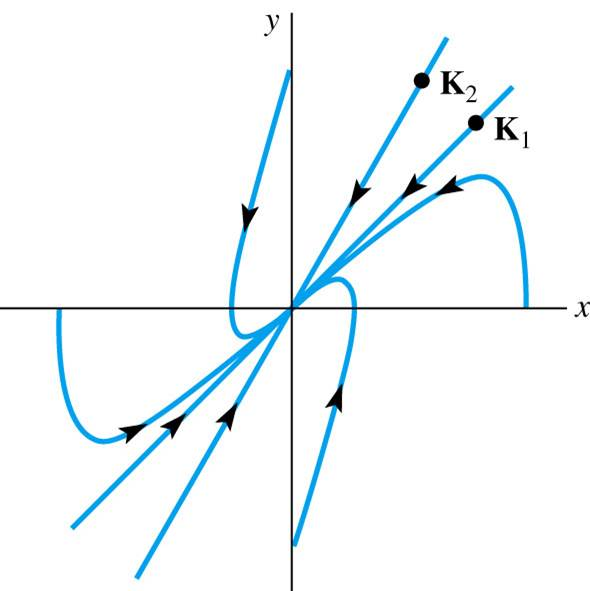
\includegraphics[scale=0.5]{nodoestable}
\caption{Nodo estable.}
\end{figure}

\item[Nodo inestable]
Si ambos autovalores son positivos, la solución se aleja del origen.
Las trayectorias de las soluciones son asintóticas a los autovalores de la matriz de coeficientes $\mathbb{A}$, excepto las soluciones con condiciones iniciales que pertenecen a las direcciones propias, entonces el sistema evoluciona sobre ellas.
%
\begin{figure}
\centering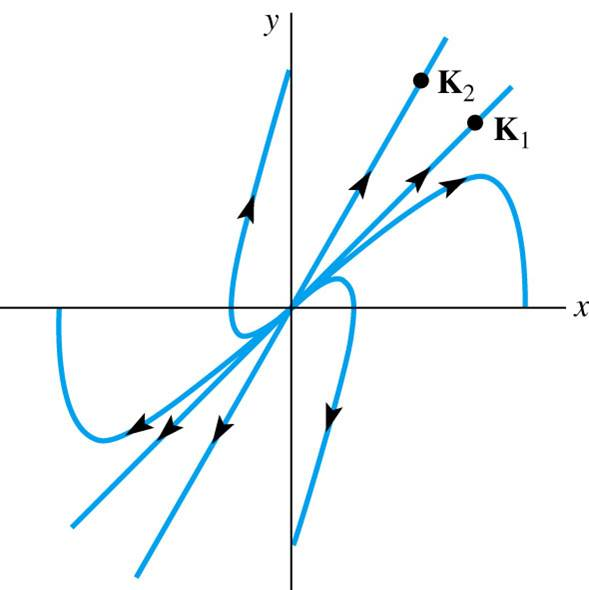
\includegraphics[scale=0.5]{nodoinestable}
\caption{Nodo inestable.}
\end{figure}

\item[Punto silla]
Si los autovalores tienen signos opuestos, la solución se aleja del origen asintóticamente a uno de los autovectores y se aproxima asintóticamente al otro, excepto las soluciones con condiciones iniciales que pertenecen a las direcciones propias, entonces el sistema evoluciona sobre ellas.
%
\begin{figure}
\centering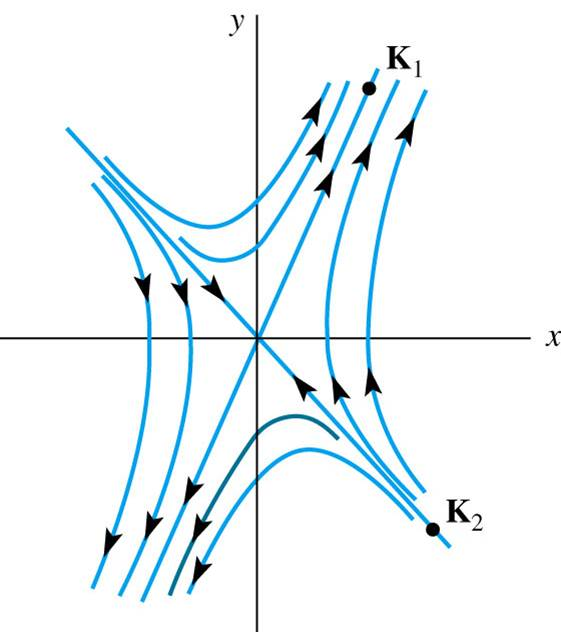
\includegraphics[scale=0.5]{silla}
\caption{Punto silla.}
\end{figure}

\item[Nodos degenerados]
Aparecen en los casos en que los autovalores o autovectores sean iguales.
Para iguales autovalores, pueden generarse todas las trayectorias radiales por combinación lineal de los autovectores. La forma de la solución será
\begin{equation}
X(t)=(c_1K_1+c_2+K_2)e^{\lambda t} \nonumber
\end{equation}
Con $c_i$ constantes, $K_i$ los autovectores y $\lambda$ un autovalor.
Si los autovalores son negativos, la solución se acerca al origen en forma radial y el nodo resulta ser estable, de lo contrario será inestable.
\begin{figure}
\centering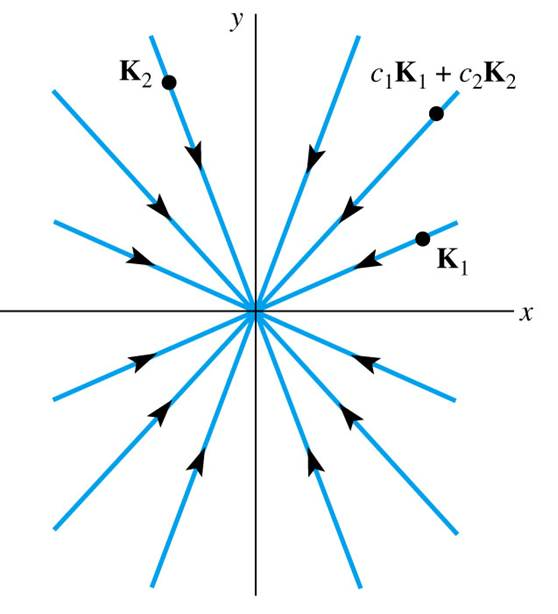
\includegraphics[scale=0.5]{nodoestabledegeneradounautovalor}
\caption{Nodo estable degenerado con autovalores negativos.}
\end{figure}
Si además tenemos iguales autovectores, la forma de la solución sería
\begin{equation}
X(t)=(c_1K+tc_2K+c_2P)e^{\lambda t} \nonumber
\end{equation}
Si los autovalores son negativos, la solución se acerca al origen y el nodo resulta ser estable, de lo contrario será inestable.
\begin{figure}
\centering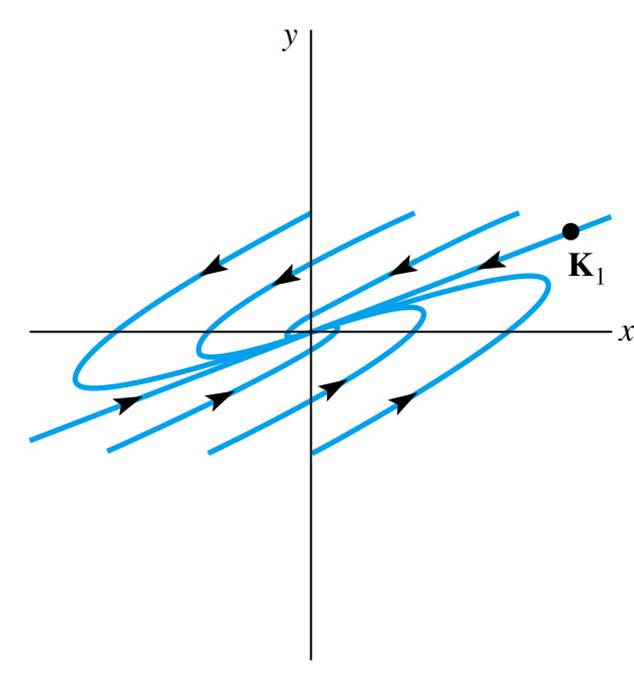
\includegraphics[scale=0.5]{nodoestabledegeneradounautovector}
\caption{Nodo estable degenerado con autovalores negativos y un solo autovector.}
\end{figure}

\item[Centro]
Si los autovalores son imaginarios puros, la solución describe elipses concéntricas que pasan por el valor inicial.
\begin{figure}
\centering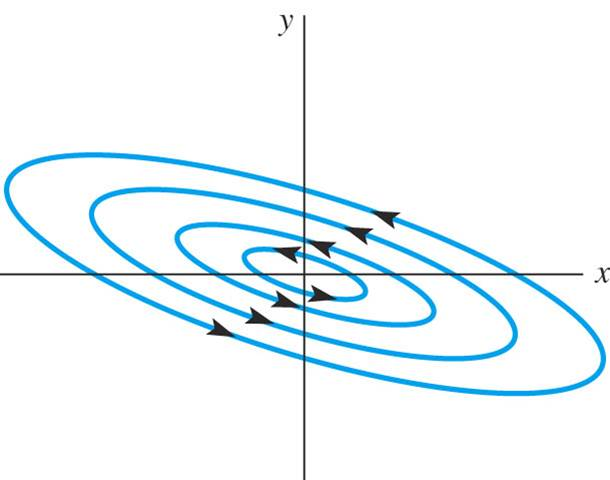
\includegraphics[scale=0.5]{centro}
\caption{Centro.}
\end{figure}

\item[Foco estable]
Si los autovalores son complejos con parte real negativa, la solución es una combinación de los casos anteriores. Será periódica conforme su parte imaginaria y se aproximará a cero según su parte real.
%
\begin{figure}
\centering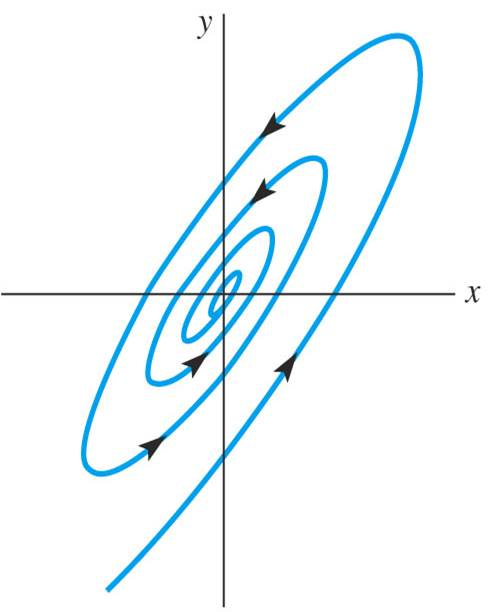
\includegraphics[scale=0.5]{focoestable}
\caption{Foco estable.}
\end{figure}

\item[Foco inestable]
Si los autovalores son complejos, la solución será periódica conforme su parte imaginaria y tenderá a infinito según su parte real.
%
\begin{figure}
\centering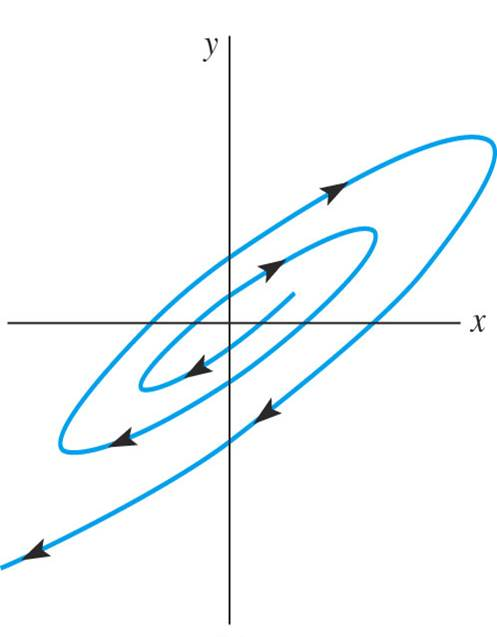
\includegraphics[scale=0.5]{focoinestable}
\caption{Foco inestable.}
\end{figure}

\end{description}

Para cualquier  sistema de ED, primero se deben hallar todos los puntos críticos del sistema. Luego, se linealiza en torno a cada uno mediante el primer término de la serie de Taylor obteniendo tantos sistemas de ecuaciones como puntos críticos tenga el sistema.
Estos sistemas son válidos en un entorno suficientemente pequeño del punto crítico.

Por ejemplo, supongamos que se necesita trazar el diagrama de fase para el péndulo físico de la Figura \ref{fig:pendulo}.
%
\begin{figure}[htpb]
	\centering
	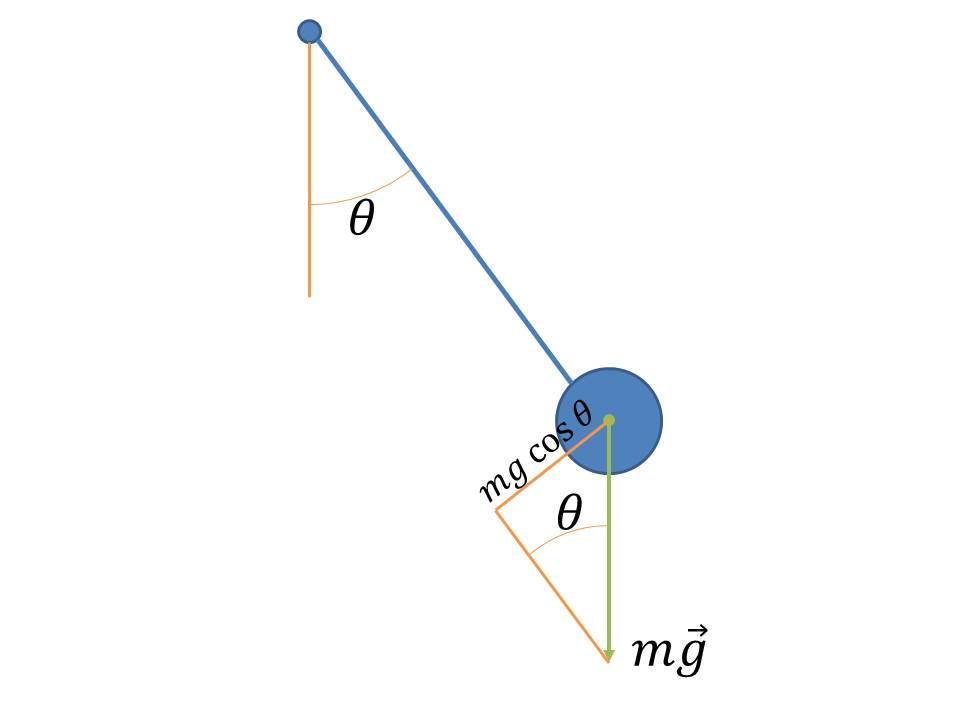
\includegraphics[width=.49\textwidth]{pendulo}
	\caption{Péndulo físico ideal.}
	\label{fig:pendulo}
\end{figure}

Primero hallamos la ecuación de la aceleración, según la Figura, la componente tangencial de la gravedad es la que acelera al cuerpo.
Tomando como referencia positiva el sentido dextrógiro, queda
%
\begin{equation}
a=mg\cos\theta - \mu v \nonumber
\end{equation}
%
en donde $\mu$ es el coeficiente de roce viscoso con el aire y $v$ la velocidad. Pero como nos interesa la aceleración angular $\alpha$ y la velocidad angular $\omega$
%
\begin{equation}
\alpha=a/l; \qquad \omega=v/l \nonumber
\end{equation}
%
siendo $l$ la longitud de la cuerda.

La aceleración angular $\alpha$ es la derivada de la velocidad angular $\omega$ que a su vez es la derivada del ángulo $\theta$
%
\begin{equation}
\alpha = \omega' = \theta'' \nonumber
\end{equation}
%
entonces el sistema de ecuaciones queda
%
\begin{equation}
\left \{
\begin{array}{rcl}
\theta' &=& \omega\\
\omega' &=& \frac{mg}{l}\cos{\theta}-\frac{\mu}{l}\omega
\end{array}
\right. \nonumber
\end{equation}

Una vez planteado el sistema de ecuaciones, el primer paso es hallar los puntos críticos del sistema.
%
\begin{equation}
\left \{
\begin{array}{rcl}
0 &=& \omega\\
0 &=& \frac{mg}{l}\cos{\theta}-\frac{\mu}{l}\omega
\end{array}
\right.
\longrightarrow
\left \{
\begin{array}{rcl}
0 &=& \omega\\
\theta &=& (2n-1)\frac{\pi}{2} \qquad n\notin\mathbb{Z}
\end{array}
\right.
\nonumber
\end{equation}

Ahora estamos en condiciones de linealizar el sistema en torno de los puntos críticos.
% 
\begin{equation}
\left \{
\begin{array}{rcl}
\theta' &=& \omega\\
\omega' &=& \frac{\partial \left(\frac{mg}{l}\cos{\theta}\right)}{\partial\theta}\Big|_{\theta = (2n-1)\frac{\pi}{2}}\theta-\frac{\mu}{l}\omega
\end{array}
\right.
=
\left \{
\begin{array}{rcl}
\theta' &=& \omega\\
\omega' &=& -\frac{mg}{l}\sin(\theta)\Big|_{\theta = (2n-1)\frac{\pi}{2}}\theta-\frac{\mu}{l}\omega
\end{array}
\right.
\nonumber
\end{equation}

Según $n$ sea par (incluyendo el cero) o impar, la ecuación lineal que representa al sistema será diferente.

Si $n$ es par o cero
%
\begin{equation}
\left \{
\begin{array}{rcl}
\theta' &=& \omega\\
\omega' &=& \frac{mg}{l}\theta-\frac{\mu}{l}\omega
\end{array}
\right.
\longrightarrow
A=
\begin{pmatrix}
0 &1 \\
\frac{mg}{l} &-\frac{\mu}{l}
\end{pmatrix}
\nonumber
\end{equation}

\begin{equation}
det(A-\lambda I)= \;
\begin{vmatrix}
-\lambda &1 \\
\frac{mg}{l} &-\frac{\mu}{l}-\lambda
\end{vmatrix}
\nonumber
=\lambda^2+\frac{\mu}{l}\lambda-\frac{mg}{l}
\nonumber
\end{equation}
los autovalores son reales y de distinto signo (punto silla).

Si $n$ es impar
\begin{equation}
\left \{
\begin{array}{rcl}
\theta' &=& \omega\\
\omega' &=& -\frac{mg}{l}\theta-\frac{\mu}{l}\omega
\end{array}
\right. \nonumber
\end{equation}

\begin{equation}
det(A-\lambda I)= \;
\begin{vmatrix}
-\lambda &1 \\
-\frac{mg}{l} &-\frac{\mu}{l}-\lambda
\end{vmatrix}
\nonumber
=\lambda^2+\frac{\mu}{l}\lambda+\frac{mg}{l}\\
\nonumber
\end{equation}
los autovalores son complejos conjugados con parte real negativa (foco estable).

La resolución numérica en Matlab (Figura \ref{fig:fase}, muestra las soluciones al sistema alineal en el espacio de estados.
Puede verse que, en los puntos críticos, la solución se aproxima a un foco o a un punto silla, según el valor de $n$.
%
\begin{figure}
\centering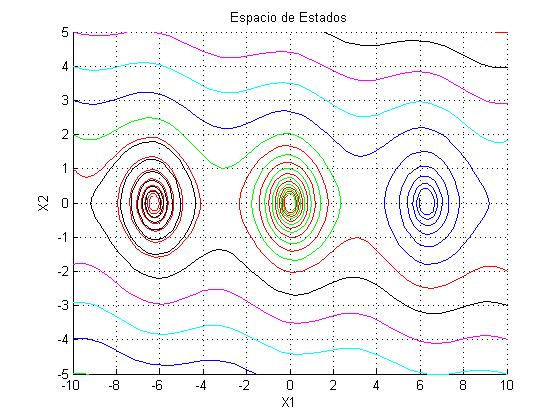
\includegraphics[scale=.7]{fase}
\caption{Diagrama de fase del péndulo físico real.}
\label{fig:fase}
\end{figure}

\section{Sistemas Caóticos}
\label{secSistCaot}

Cuando se miden variables físicas, no es muy extraño encontrar que el plano de fases tiene un comportamiento similar al de la Figura \ref{fig:Secuencia-OK_2}.
Puede verse que las trayectorias se cortan en el plano de fase, lo que indica que el sistema tiene un orden mayor que dos.
Otra observación que se puede hacer es que las trayectorias no se repiten, es decir que, aunque la oscilación persiste, no aparece un ciclo con trayectoria definida.
Esta última propiedad clasifica al sistema que se está midiendo como caótico.

\begin{figure}
\centering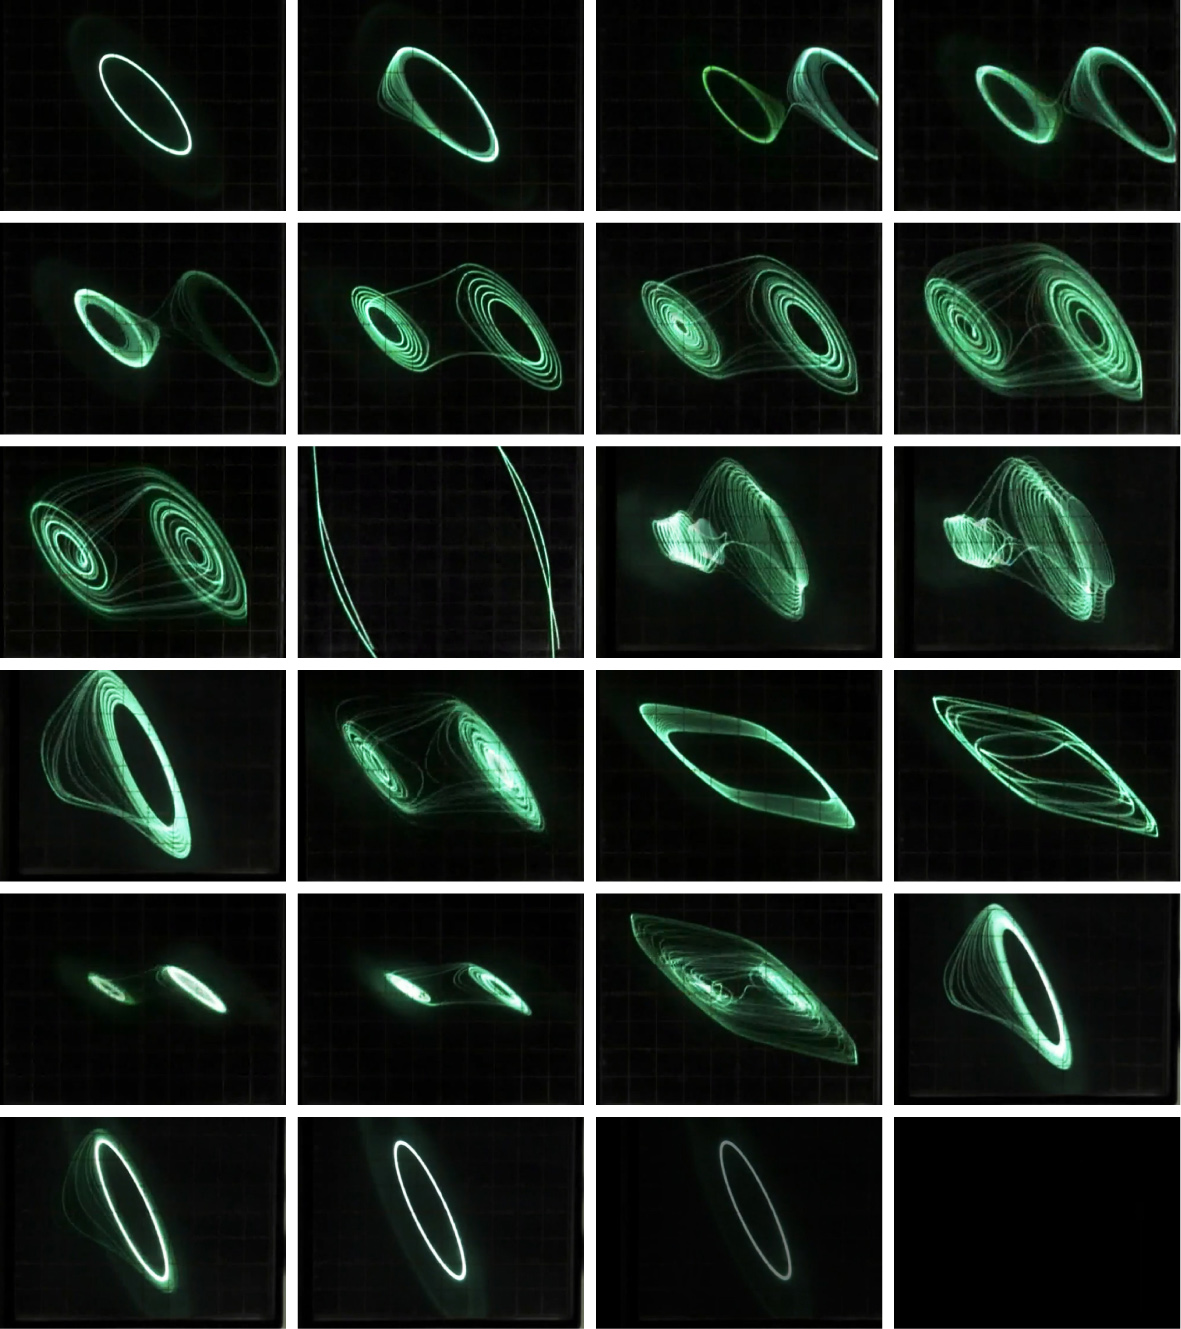
\includegraphics[width=0.8\textwidth]{Secuencia-OK_2}
\caption{Salidas de tensión de dos variables de un circuito oscilador.}
\label{fig:Secuencia-OK_2}
\end{figure}

El teorema de existencia y unicidad de las soluciones a un sistema de ecuaciones garantiza que, si una función $f$ es continuamente diferenciable, los campos vectoriales sobre el espacio de fases son suaves y cada punto de este espacio tiene solución única.
La existencia de este teorema tiene un corolario importante: trayectorias diferentes nunca se intersectan.
Como consecuencia de esto, las trayectorias sobre el plano de fases quedan restringidas a: un nodo estable o inestable, centro, foco estable o inestable y puerto.
Entonces queda claro que un sistema continuo con derivada continua debe tener dimensión mayor o igual a tres para que pueda ser caótico, además, la trayectoria en el espacio de fases debe ocupar un dominio restringido.

Para describir analíticamente el comportamiento de este tipo de sistemas en torno a ciertos puntos de interés podemos hacer uso del álgebra lineal.
Lo que sigue son tres ejemplos de aplicaciones para atractores caóticos.

El primer y más común ejemplo es el sistema de Lorenz, que está descrito por el siguiente sistema de ecuaciones diferenciales \cite{Lorenz1963}:
\begin{equation}\label{eq:lorenz}
\left \{
\begin{array}{rcl}
x_1' &=& \sigma (x_1-x_2)\\
x_2' &=& -x_1x_3+\rho x_3-x_2\\
x_3' &=& x_1x_2-\beta x_3
\end{array}
\right.
\end{equation}
En donde $\sigma$, $\rho$ y $\beta$ son parámetros del sistema, la dinámica será caótica según que combinación de estos valores elijamos.

El sistema de Lorenz tiene tres puntos de equilibrio, $E$, $E^+$ y $E^-$: el primer punto de equilibrio $E$ está situado en el origen (0,0,0) y los otros dos tienen respectivamente como coordenadas,
\begin{equation}
(x_1^\pm,x_2^\pm,x_3)=\left(\pm \sqrt{\beta(\rho-1)},\pm \sqrt{\beta(\rho-1)},\rho - 1\right) \nonumber
\end{equation}


Un comportamiento físico interesante de este sistema ocurre cuando variamos el parámetro de control $\rho$.
Cuando $\rho<1$, todas las órbitas del campo vectorial dado por la Ecuación \ref{eq:lorenz} tienden al punto fijo situado en el origen.
A medida que se va incrementando más allá de la unidad, el origen pasa a ser inestable dando lugar a dos puntos fijos, estables, y simétricos $E^+$ y $E^-$. Para todo $\rho<1$, la geometría del comportamiento asintótico del sistema es la misma ya que todas las condiciones iniciales tienden al origen E.

Para $\rho>1$, se observan dos comportamientos.
El primero, asociado a valores de $\rho$ menores que un cierto valor de umbral $\rho_u=(\sigma(\sigma+\beta)+3\sigma)/(\sigma-\beta-1)$ , valor para el cual los puntos de equilibrio $E^+$ y $E^-$ pierden su estabilidad.
Dentro de este rango de valores del parámetro todas las órbitas terminan en uno de los dos puntos de equilibrio dependiendo de las condiciones iniciales.

Cuando $\rho>\rho_u$, la situación cambia drásticamente.
Los dos puntos fijos pasan a ser inestables y nuevos comportamientos pueden surgir.
Para estudiar estos comportamientos se considera el análisis dinámico del sistema de Lorenz \ref{eq:lorenz}. 
La linealización en la proximidad del origen nos proporciona los siguientes autovalores:
\begin{equation}
\lambda = -\beta;\\
\lambda_\pm = \frac{1}{2} \left[-(\sigma+1) \pm \sqrt{(\sigma+1)^2+4\sigma(\rho-1)} \right] \nonumber
\end{equation}
 asociados a la matriz Jacobiana:
\begin{equation}
\begin{pmatrix}
-\sigma &\sigma &0 \\
\rho &-1 &0 \\
0 &0 &-\beta
\end{pmatrix}
\nonumber
\end{equation}

Los autovalores  $\lambda$ y $\lambda_-$ son siempre negativos; el autovalor $\lambda_+$ cambia de negativo a positivo cuando $\rho$ pasa por el valor 1.

De modo similar, la linealización del sistema \ref{eq:lorenz} en la proximidad del punto de equilibrio $E^+$ nos proporciona los siguientes autovalores:
\begin{equation}
\lambda^3+\lambda^2(\sigma+\beta+1)+\lambda\beta(\sigma+\rho)+2\sigma\beta(\rho-1)=0 \nonumber
\end{equation}
asociados a la matriz Jacobiana:
\begin{equation}
\begin{pmatrix}
-\sigma &\sigma &0 \\
\rho-x_3 &-1 &-x_1 \\
x_2 &x_1 &-\beta
\end{pmatrix}
\nonumber
\end{equation}
tiene un autovalor real negativo $\lambda$ combinado con dos autovalores imaginarios puros, $\lambda_\pm = \pm j \alpha$, si $\rho < \rho_h$.
La linealización del sistema \ref{eq:lorenz} en la proximidad del punto de equilibrio $E^+$ es un problema simétrico a este.

En la Figura \ref{fig:lorenz} puede verse la evolución de las soluciones al sistema de Lorenz.
%
\begin{figure}
\centering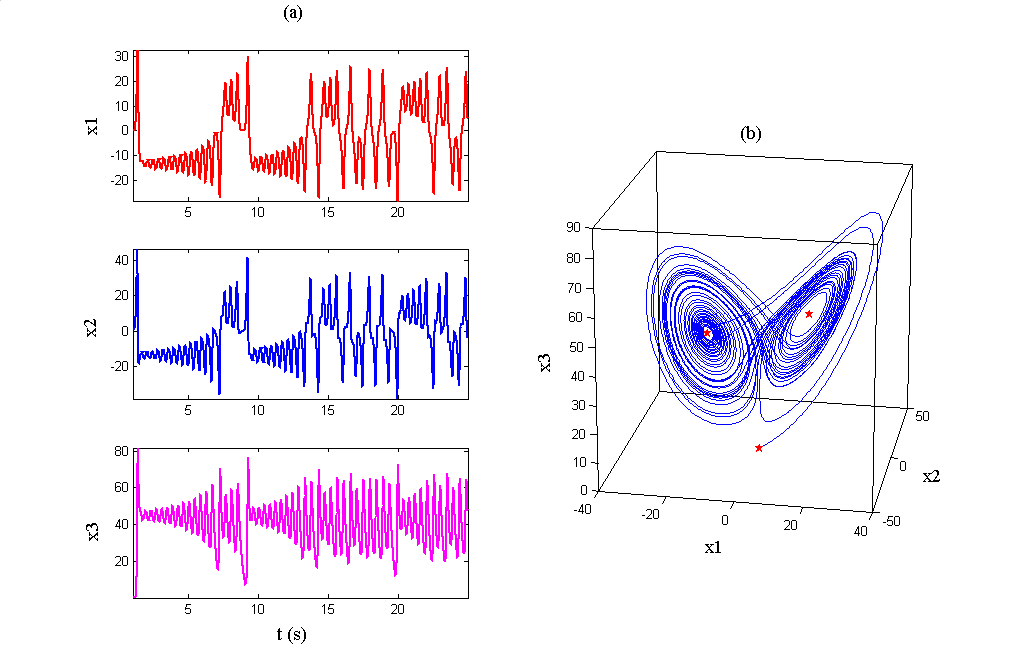
\includegraphics[scale=.4]{lorenz}
\caption{(a) Evolución temporal de las tres variables del sistema de Lorenz. (b) Disposición de sus puntos de equilibrio (estrellas rojas) con respecto a su atractor en el espacio de estados.}
\label{fig:lorenz}
\end{figure}

El sistema de Rössler está descrito por el siguiente sistema de ecuaciones diferenciales
\begin{equation}\label{eq:rossler}
\left \{
\begin{array}{rcl}
x_1' &=& x_2-x_3\\
x_2' &=& x_1x_3+ax_2\\
x_3' &=& b+(x_1+c)x_3
\end{array}
\right.
\end{equation}
en donde $a$, $b$ y $c$ son parámetros del sistema.

El sistema de Rössler tiene dos puntos de equilibrio, $E^+$ y $E^-$ que existen sólo cuando $\Delta = c^2-4ab > 0$ y cuyas coordenadas están dadas respectivamente por,
\begin{equation}
(x_1^\pm,x_2^\pm,x_3^\pm)=\left( \frac{1}{2} (c \pm \sqrt{\Delta}),-\frac{1}{2a} (c \pm \sqrt{\Delta}),\frac{1}{2a} (c \pm \sqrt{\Delta})\right) \nonumber
\end{equation}
 
La linealización del sistema \ref{eq:rossler} en la proximidad de los puntos de equilibrio proporciona los siguientes autovalores:

\begin{equation}
a \lambda^3 - \lambda^2 a (x_1-c)-\lambda(x_3-1)+ax_3+(x_1-c)=0 \nonumber
\end{equation}
 asociados a la matriz Jacobiana
 
\begin{equation}
\begin{pmatrix}
0 &\-1 &-1 \\
1 &a &0 \\
x_3^\pm &0 &x_1^\pm-c
\end{pmatrix}
\nonumber
\end{equation}
de donde se deduce que fijando los parámetros $a$ y $b$ y variando $c$ nos encontramos con dos escenarios diferentes, podemos tener un autovalor real negativo y dos complejos conjugados con parte real positiva, o un autovalor real negativo y dos complejos conjugados con parte real negativa.
Para valores pequeños de c, el atractor de Rössler consiste en una órbita periódica o ciclo límite que tiene un sólo mínimo local.
A medida que vamos incrementando el parámetro c, el ciclo límite va duplicando su período y como consecuencia, sus mínimos locales hasta alcanzar un límite en el cual las trayectorias nunca se repiten, lo que corresponde al atractor caótico de Rössler. 

En la Figura \ref{fig:rossler_parametro} pueden verse la evolución de las variables $x_1$ y $x_2$ en el sistema de Rössler para distintos valores del parámetro $c$.
En la Figura \ref{fig:rossler}, se puede ver la evolución de las tres variables para un parámetro fijo.
%
\begin{figure}
\centering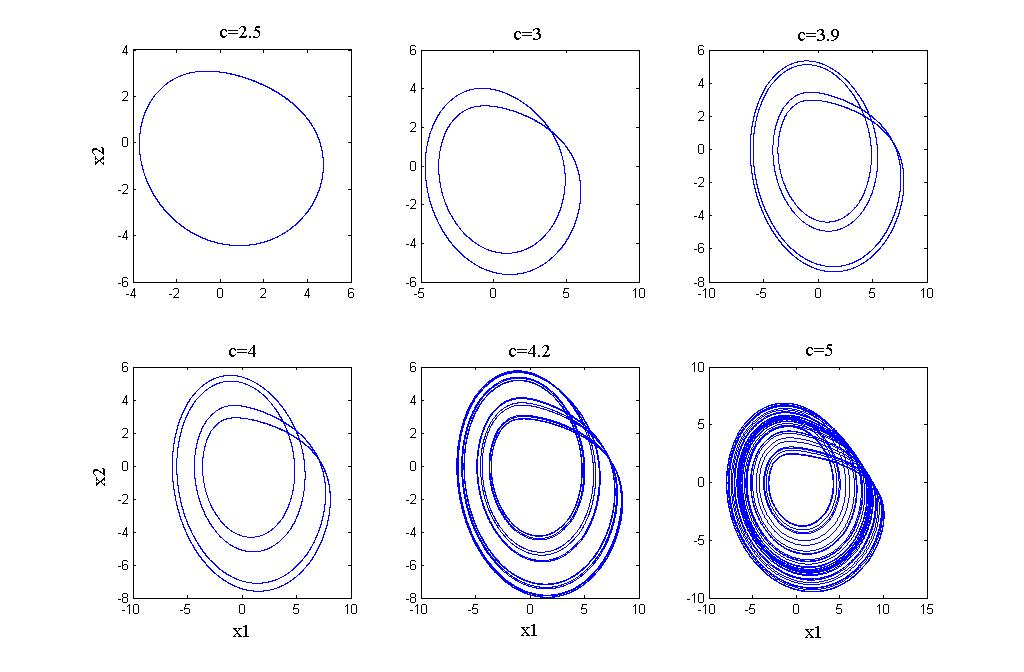
\includegraphics[scale=.5]{rossler_parametro}
\caption{Proyecciones del atractor de Rössler en el plano  para diferentes valores del parámetro c.}
\label{fig:rossler_parametro}
\end{figure}
%
\begin{figure}
\centering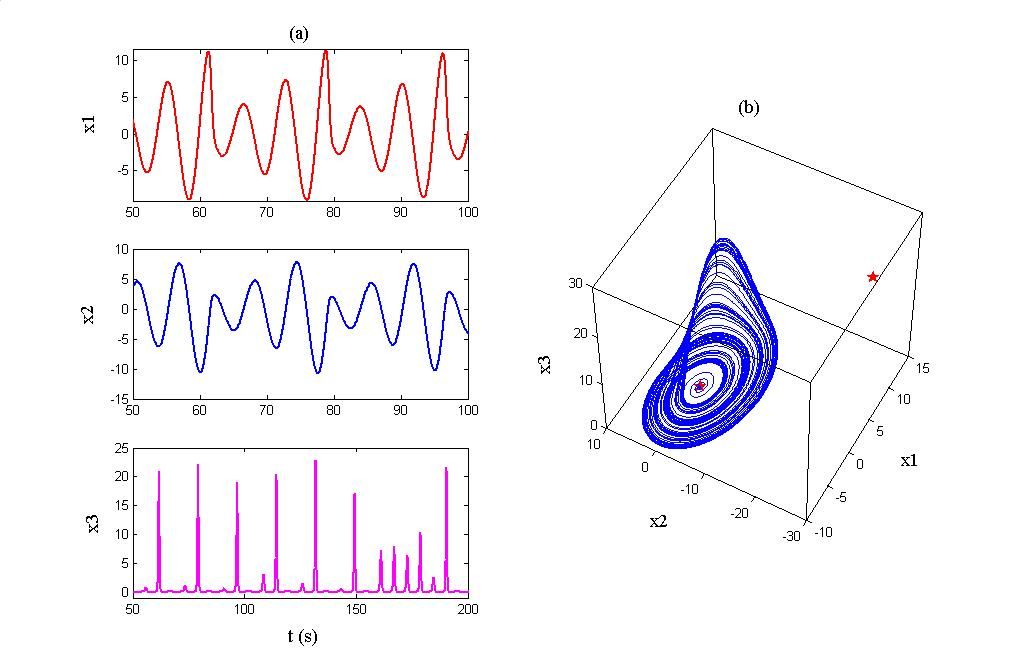
\includegraphics[scale=.5]{rossler}
\caption{(a) Evolución temporal de las tres variables del sistema de Rössler. (b) Disposición de sus puntos de equilibrio (estrellas rojas) con respecto a su atractor en el espacio de estados.}
\label{fig:rossler}
\end{figure}

El sistema de Chua está descrito por el siguiente sistema de ecuaciones diferenciales:
\begin{equation}\label{eq:chua}
\left \{
\begin{array}{rcl}
x_1' &=& \alpha x_2- \alpha x_1^3- \alpha c x_1\\
x_2' &=& x_1 + x_3 - x_2\\
x_3' &=& -\beta x_2
\end{array}
\right.
\end{equation}

Este sistema tiene tres puntos de equilibrio, $E$, $E^+$ y $E^-$: el primer punto de equilibrio $E$ está situado en el origen (0,0,0) y los otros dos tienen respectivamente como coordenadas,
\begin{equation}
(x_1^\pm,x_2^\pm,x_3)=\left(\pm \sqrt{-c}, 0,\pm \sqrt{-c}\right) \nonumber
\end{equation}
Los puntos de equilibrio existen sólo para valores positivos del parámetro c.

La linealización del sistema \ref{eq:chua} en la proximidad de los puntos de equilibrio proporciona los siguientes autovalores:

\begin{equation}
\lambda^3 + \lambda^2 \alpha (\alpha c+1)+\lambda(\alpha c-\alpha+\beta)+ax_3+\alpha\beta c=0 \nonumber
\end{equation}
asociados a la matriz Jacobiana
\begin{equation}
\begin{pmatrix}
-\alpha c &\alpha &0 \\
1 &-1 &1 \\
0 &-\beta &0
\end{pmatrix}
\nonumber
\end{equation}
donde podemos detectar un punto de bifurcación para $\alpha=0$ en el cual el autovalor real negativo pasa a ser positivo provocando la inestabilidad del punto de equilibrio $E$ que permanece inestable para una amplia gama de valores del parámetro $\alpha$.

En la Figura \ref{fig:chua}, puede verse la evolución de las tres variables de estado para este sistema.
%
\begin{figure}
\centering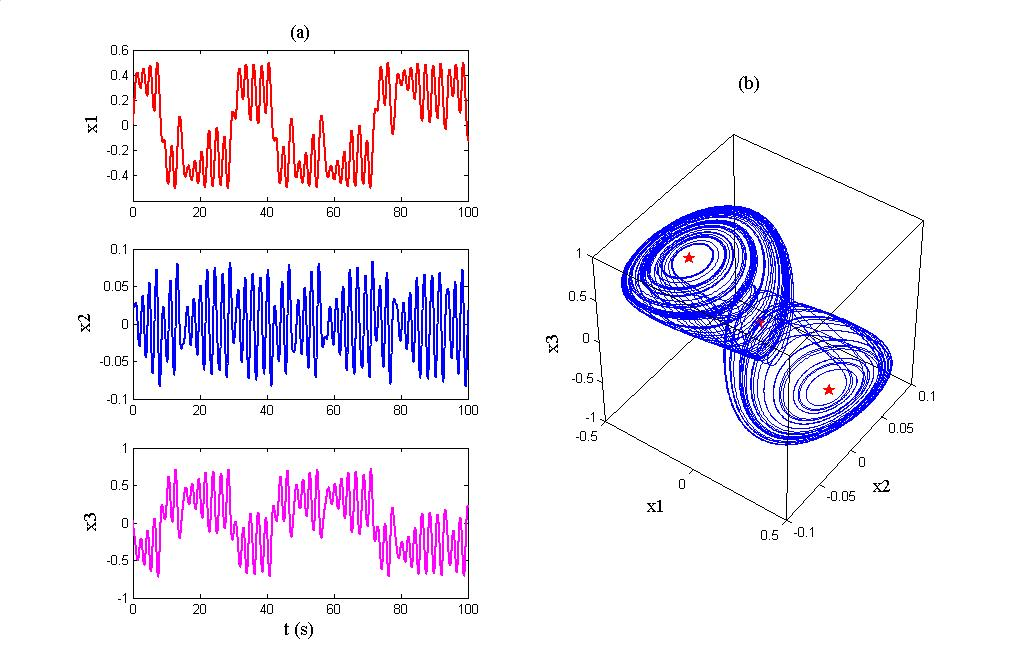
\includegraphics[scale=.5]{chua}
\caption{(a) Evolución temporal de las tres variables del sistema de Chua. (b) Disposición de sus puntos de equilibrio (estrellas rojas) con respecto a su atractor en el espacio de estados.}
\label{fig:chua}
\end{figure}

\section{Mapas Caóticos}

Los mapas son una relación de recurrencias, cuya salida puede presentar un comportamiento caótico. Dentro de la gran familia de mapas unidimensionales destacamos los mapas Tent y Logístico, que son utilizados posteriormente en esta tesis.

\subsection{Mapa Logístico}

El mapa Logístico es un claro ejemplo de cómo a partir de ecuaciones dinámicas lineales muy simples puede surgir un comportamiento caótico complejo. Su representación matemática es una relación de recurrencia polinomial de grado 2:
\begin{equation}\label{eqLogistico}
x_{n+1} = rx_n(1-x_n)
\end{equation}
en donde $r$ es un parámetro del sistema.

La evolución de las iteraciones de este mapa exhibe una gran sensibilidad a las condiciones iniciales, dependiendo del parámetro $r$. Para el intervalo $3.57 \leq r \leq 4$ este mapa presenta comportamiento caótico.
Su representación en el plano $x_{n+1}$ vs. $x_n$ se ve en la Figura \ref{figLogisticMap} para tres valores del parámetro $r = {2, 3, 4}$.
También podemos ver su diagrama de bifurcaciones en \ref{figLogisticBifurcations}, los tres valores del parámetro elegidos se resaltan en esta Figura.
\begin{figure}
	\centering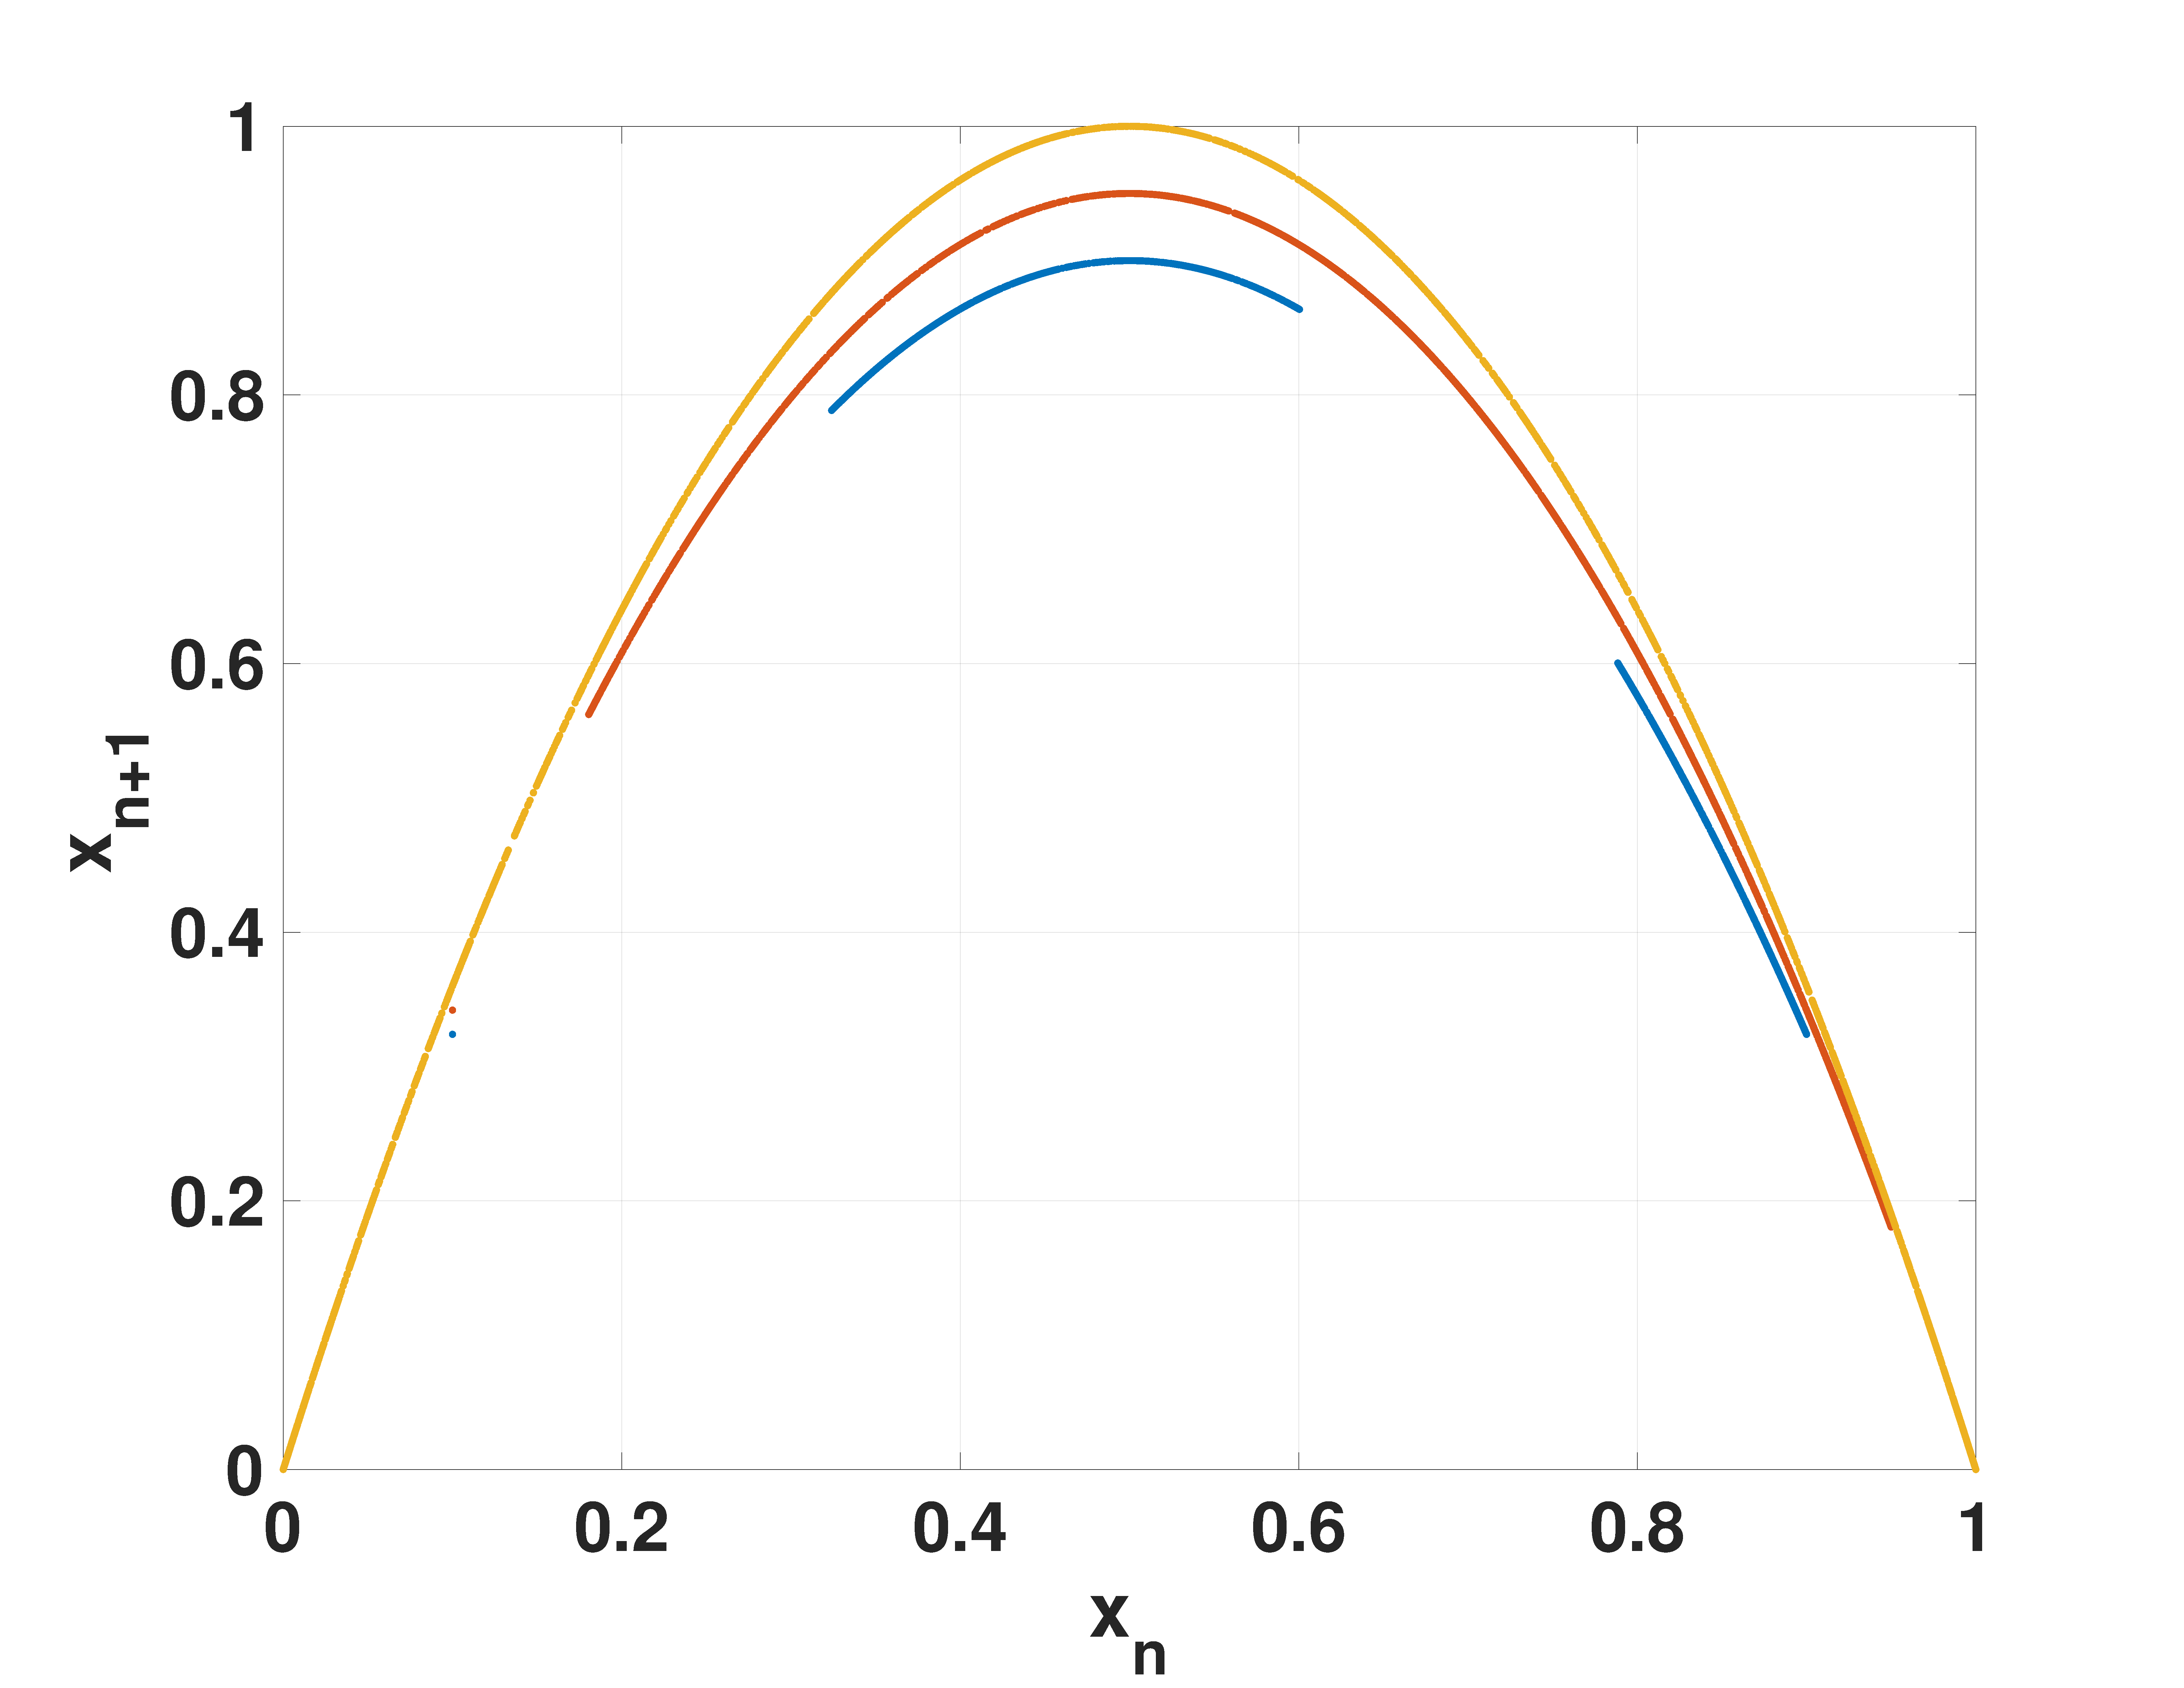
\includegraphics[width=.75\textwidth]{LogisticMap}
	\caption{Mapa Logístico para tres parámetros distintos, $r = {2, 3, 4}$}
	\label{figLogisticMap}
\end{figure}
\begin{figure}
	\centering\includegraphics[width=.75\textwidth]{LogisticBifurcations}
	\caption{Diagrama de bifurcaciones para el mapa Logístico, con valores de parámetro $2.8 \leq r \leq 4$.}
	\label{figLogisticBifurcations}
\end{figure}

\subsection{Mapa Tent}

El mapa Tent está definido por la ecuación de recurrencias:
\begin{equation}\label{eqTent}
x_{n+1} =
\begin{cases}
u~x_n &, \textrm{si } 0\leq x_n\leq 1/u\\
\frac{u}{1-u}~(1-x_n) &, \textrm{si } 1/u< x_n\leq 1 
\end{cases}
\end{equation}
%
con $x_n$ y $u \in \mathbb{R}$.

El nombre ``Tent'' viene de su representación en el plano $x_{n+1}$ vs. $x_n$ que se ve en la Figura \ref{figTentMap}, en donde el parámetro toma tres valores, $u = {4, 2, 4/3}$.
Cuando este parámetro es distinto de $2$, se dice que el mapa es un \textit{skew Tent}.
\begin{figure}
	\centering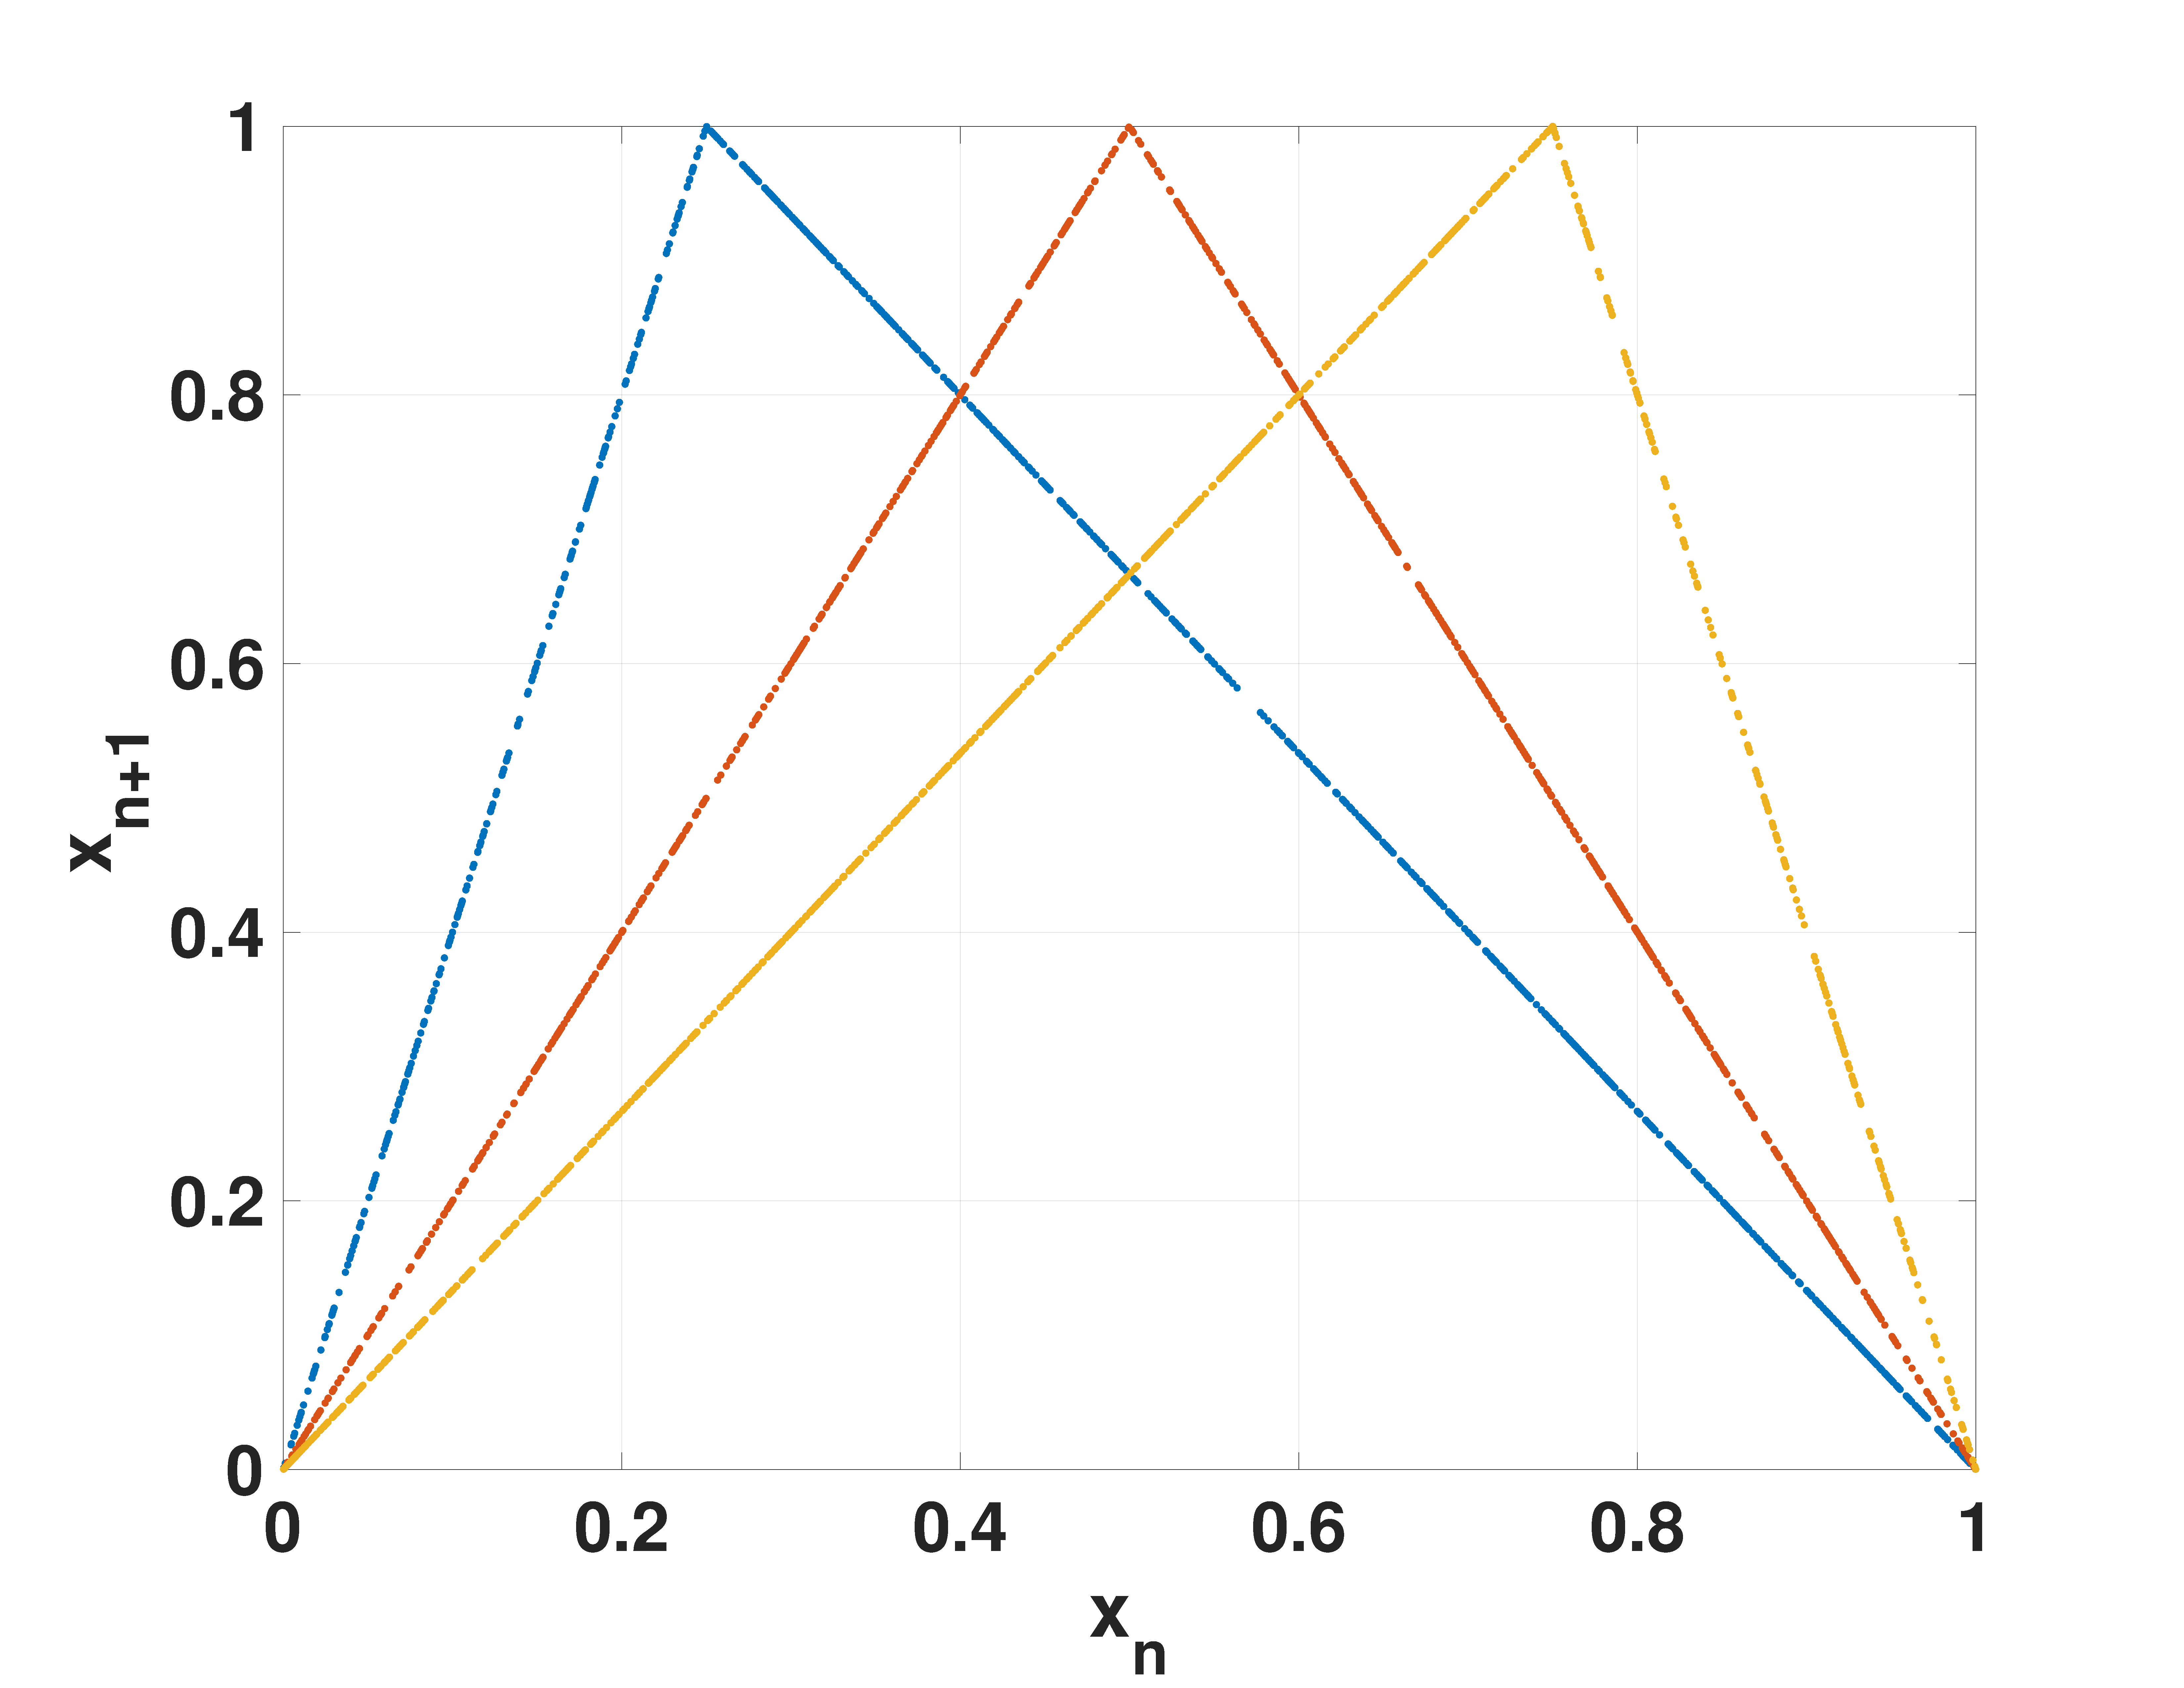
\includegraphics[width=.75\textwidth]{TentMap}
	\caption{Mapa Tent para tres parámetros distintos, $u = {4, 2, 4/3}$}
	\label{figTentMap}
\end{figure}

Este mapa tiene la característica de que para $r = 2$ sus propiedades estadísticas son ideales, cuando se las calcula teóricamente mediante el operador de Perron-Frobenious \cite{Lasota1994, Lasota1973}, es decir analíticamente.
Sin embargo, a la hora de la implementación en un medio digital, todas sus iteraciones pueden ser representadas con una operación de acarreo de bits desde la izquierda, lo que provoca que converja rápidamente a cero.
Este hecho está muy bien explicado en \cite{Li2004}.

\subsection{Mapas Cuadráticos Bidimensionales}
\label{ssecQMaps}

La familia de mapas cuadráticos bidimensionales que estudiamos aquí es modelada por un par de ecuaciones cuadráticas acopladas:
%
\begin{equation}\label{eq:mapaSprott}
\left\{\begin{aligned}
x_{n+1}&=a_1+a_2 x_n+a_3 x_n^2+a_4 x_n y_n+a_5 y_n+a_6 y_n^2\\
y_{n+1}&=a_7+a_8 x_n+a_9 x_n^2+a_{10} x_n y_n+a_{11} y_n+a_{12} y_n^2
\end{aligned}
\right.
\end{equation}
%
donde $(x, y)$ son las variables de estado y $A = \{a_i, i = 1, \dots, 12 \}$ son los parámetros.
La principal característica de este sistema es que presenta múltiples atractores caóticos en función del punto seleccionado en el espacio de parámetros.
El espacio de parámetros de $12D$ generado por los coeficientes $A$ es muy difícil de explorar.

Las razones para estudiar este sistema en particular son dos:
%
\begin{enumerate}
	\item Usando la aritmética de punto flotante con un barrido automático de parámetros $a_i$ y una gran cantidad de puntos en el espacio del parámetro (alrededor de $6\cdot10 ^ {16}$), Sprott pudo detectar varios atractores en régimen caótico permanente.
	Es decir, este sistema tiene la característica de modificar su atractor según los valores que tomen sus 12 coeficientes reales.
	También encontró una relación entre la dimensión de correlación y los exponentes de Lyapunov, con su estética visual, un tema interesante para la generación automática de arte.
	\item Es posible emplear estos atractores en una amplia variedad de aplicaciones electrónicas, como la generación de nuevos sistemas de encriptación, ya sea reemplazando el S-box en AES \cite{Ahmad2013, Hussain2013}, o incluso desarrollando nuevos algoritmos \cite{Machado2004, Smaoui2009}.
\end{enumerate}

Tres de estos atractores caóticos se muestran juntos en la Figura \ref{fig:atractoresQMaps}.
Sus juegos de parámetros $A_i$ son:	
%
\begin{eqnarray}
A_1 &=& \{-0.7,-0.4,0.5,-1.0,-0.9,-0.8,0.5,0.5,0.3,0.9,-0.1,-0.9\},\nonumber\\
A_2 &=& \{-0.6,-0.1,1.1,0.2,-0.8,0.6,-0.7,0.7,0.7,0.3,0.6,0.9\}, \nonumber\\
A_3 &=& \{-0.1,0.8,-0.7,-1.1,1.1,-0.7,-0.4,0.6,-0.6,-0.3,1.2,0.6\}.\nonumber\\
\end{eqnarray}
%
Como se puede ver en la Figura, es posible obtener salidas muy diferentes simplemente modificando el valor de los parámetros y manteniendo la estructura del sistema.
En una implementación electrónica, esto sería equivalente a poder variar la salida manteniendo la estructura del hardware y modificando los parámetros a través de, por ejemplo, una entrada.
%
\begin{figure}
	\centering
	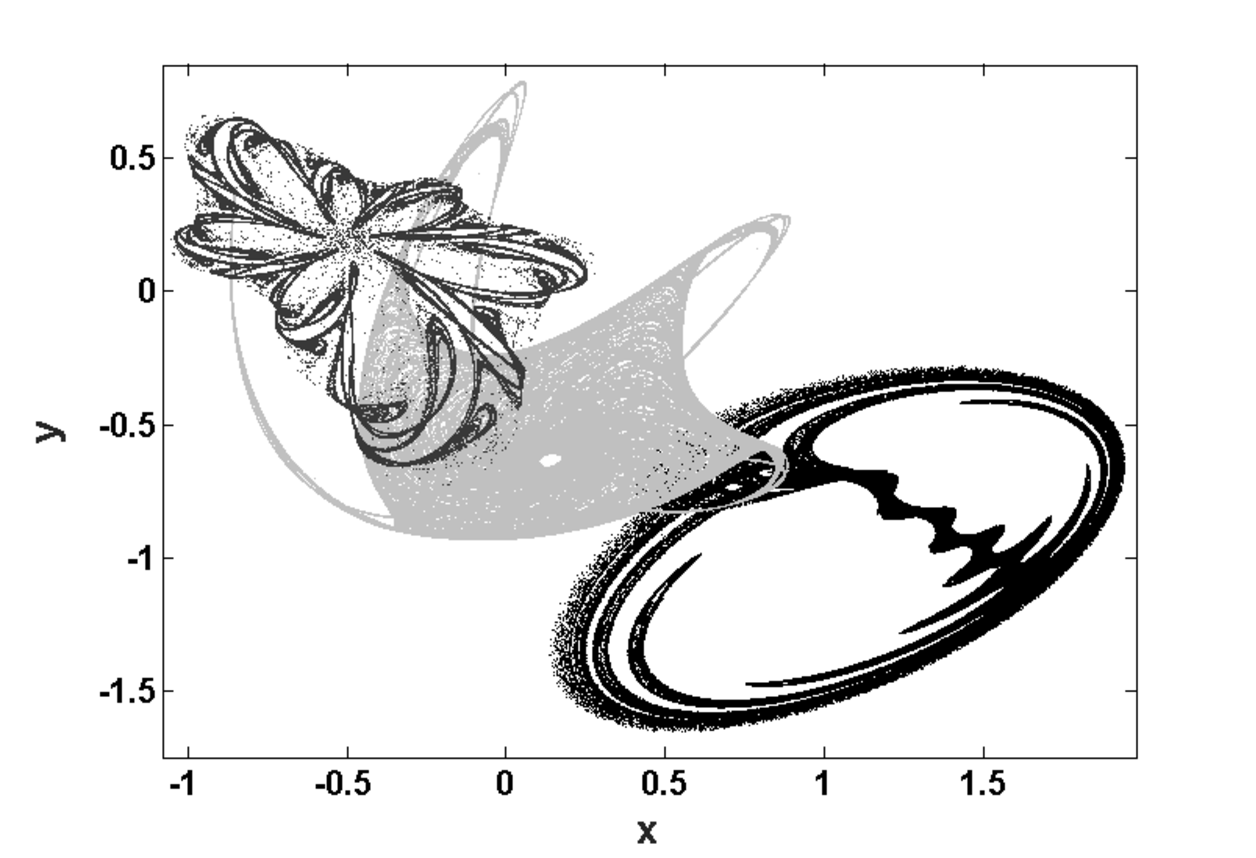
\includegraphics[width=1\columnwidth]{atractoreslindos}\\
	\caption{Atractores de sistema de mapas cuadráticos bidimensionales evaluado con tres juegos diferentes de parametros.}\label{fig:atractoresQMaps}
\end{figure}

Las Figuras \ref{fig:atractores3592}.a a \ref{fig:atractores3592}.d muestran los mismos tres atractores $A_1$ a $A_3$ de la Figura \ref{fig:atractoresQMaps} junto a un atractor con $A_4 = \{-1, 0.9, 0.4, -0.2, -0.6,-0.5, 0.4, 0.7, 0.3, -0.5, 0.7, -0.8\}$, superpuestos con sus dominios de atracción (en gris).
Las áreas blancas de cada Figura corresponden a aquellas condiciones iniciales que generan trayectorias divergentes del sistema (semillas inútiles con respecto a su uso como PRNG).	
%
\begin{figure}
	\centering
	\begin{subfigure}[b]{0.49\textwidth}
		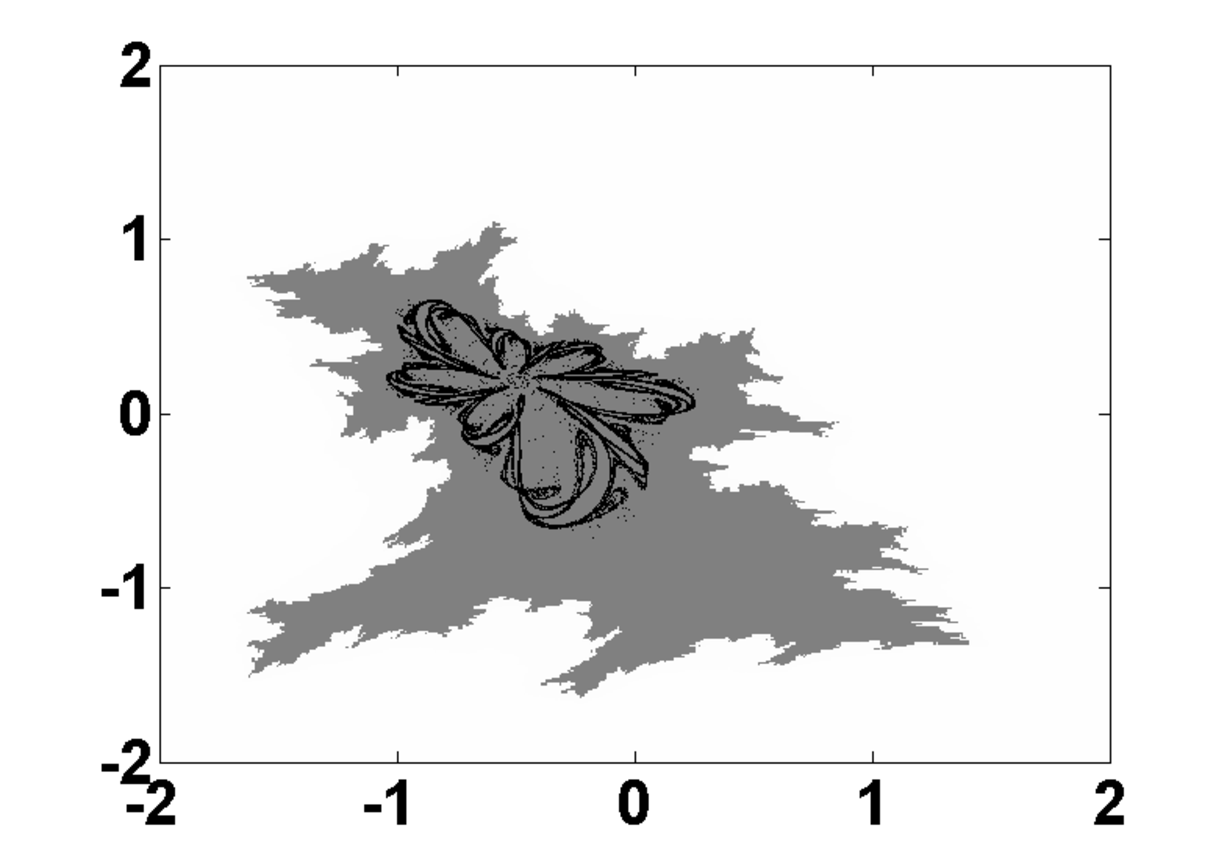
\includegraphics[width=\textwidth]{Atractor3_condominio}
		\caption{$\{a_i\}=A_1$.}
	\end{subfigure}
	\hfill 
	\begin{subfigure}[b]{0.49\textwidth}
		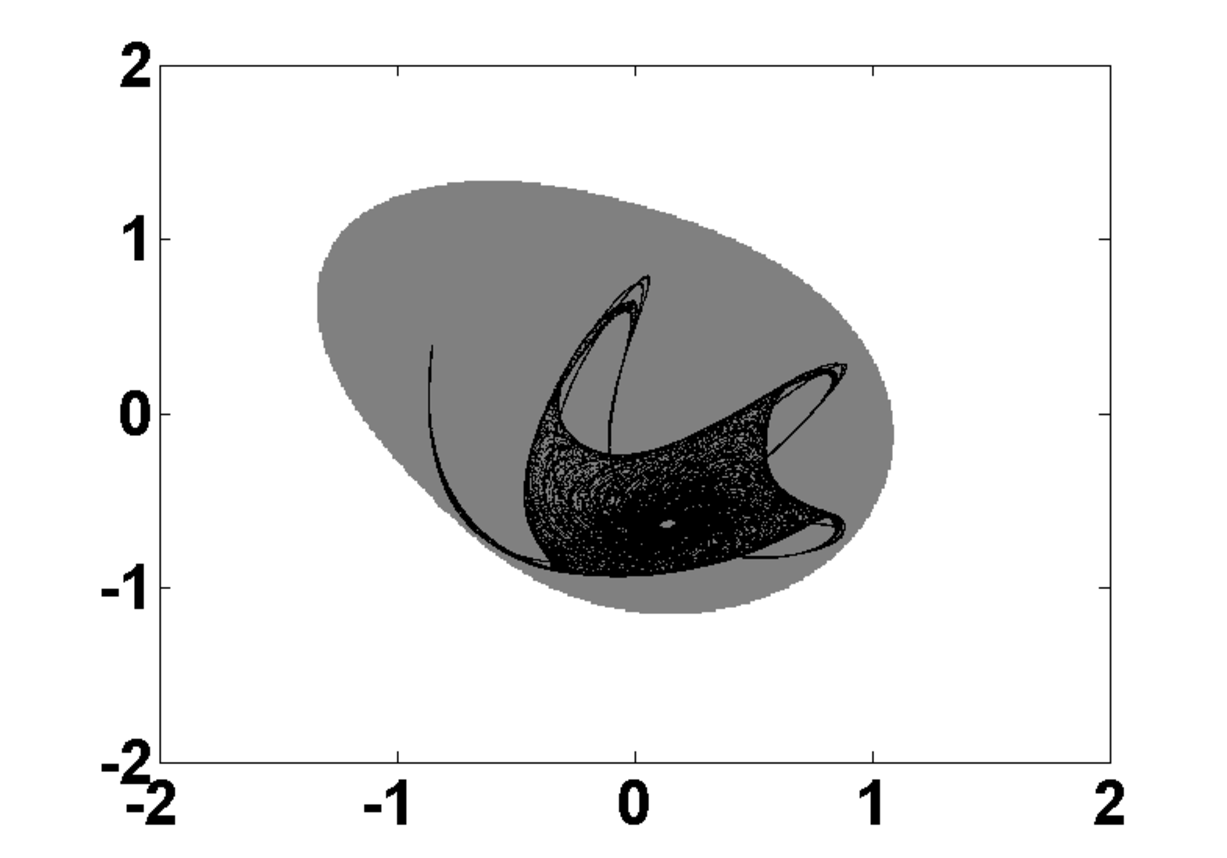
\includegraphics[width=\textwidth]{Atractor5_condminio}
		\caption{$\{a_i\}=A_2$.}
	\end{subfigure}
	\hfill 
	\begin{subfigure}[b]{0.49\textwidth}
		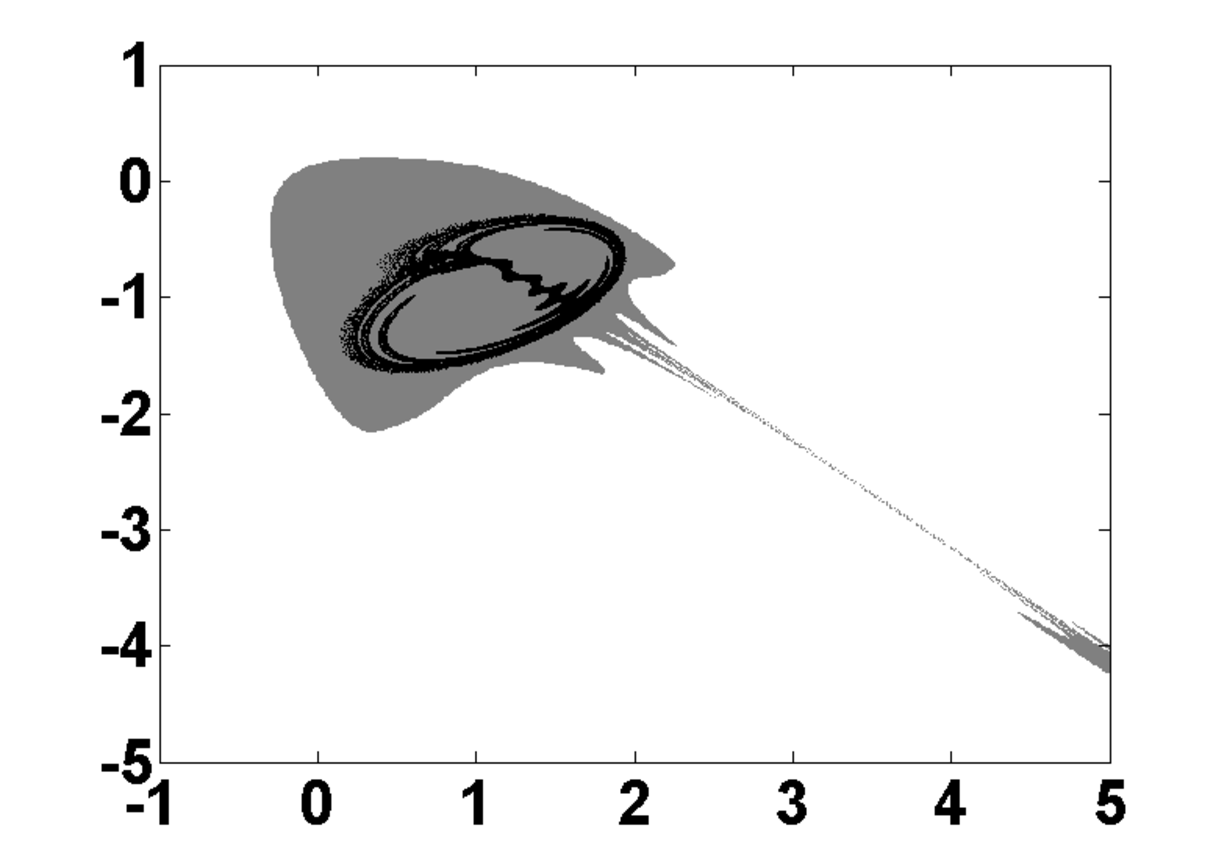
\includegraphics[width=\textwidth]{Atractor9_condominio}
		\caption{$\{a_i\}=A_3$.}
	\end{subfigure}
	\hfill  
	\begin{subfigure}[b]{0.49\textwidth}
		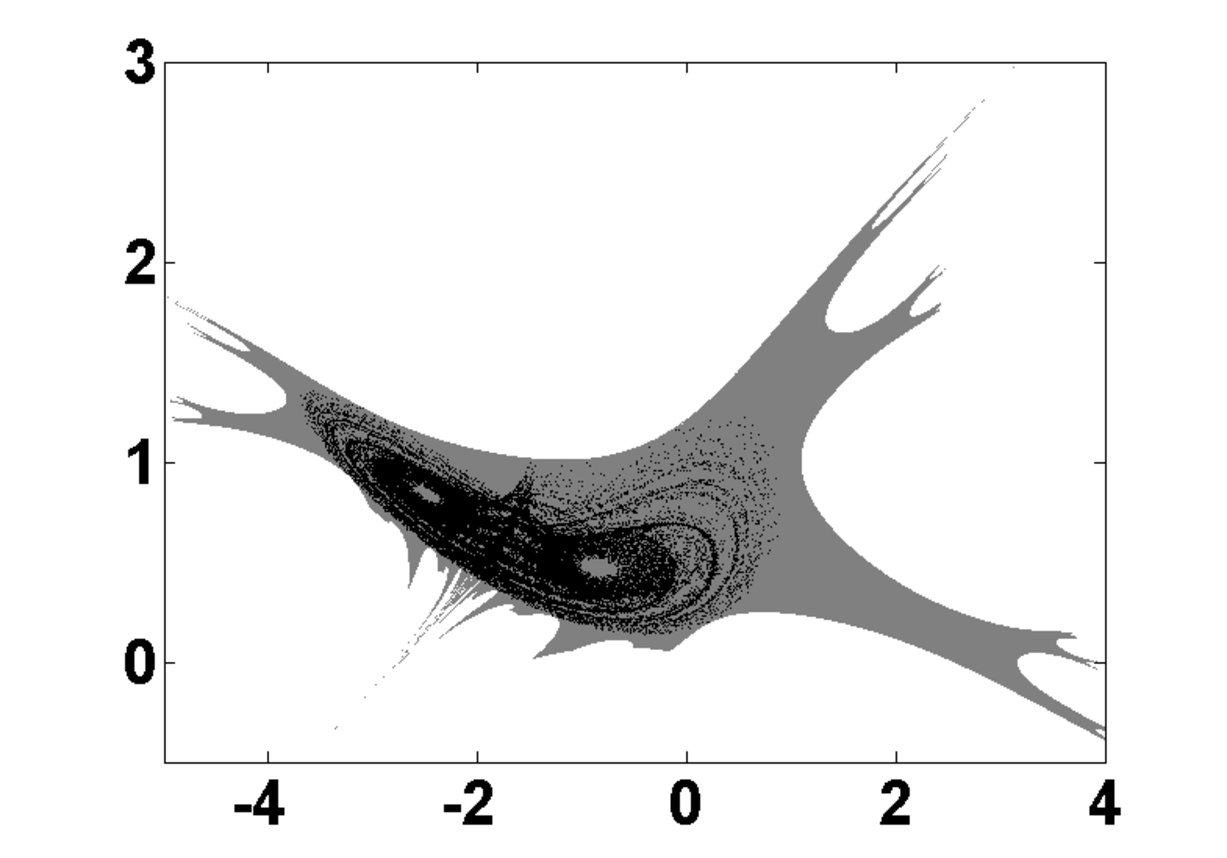
\includegraphics[width=\textwidth]{Atractor2_condominio}
		\caption{$\{a_i\}=A_4$.}
	\end{subfigure}
	\caption{Cuatro atractores caóticos y sus respectivos dominios de atracción.}
	\label{fig:atractores3592}
\end{figure}

\section{El problema de la Aritmética Discreta}

Cuando un sistema con MLE positivo es implementado utilizando Aritmética discreta, su comportamiento puede variar respecto del sistema original en aritmética de números reales. En un sistema como este, las pequeñas perturbaciones son amplificadas exponencialmente, y los ``saltos'' en las trayectorias provocados por la aritmética pueden ser considerados como tales.

Al iterar mapas caóticos, después de un transitorio que depende del parámetro de mezcla ($r_{mix}$), la secuencia generada limita en un punto o colección de puntos llamado atractor.
Un mapa caótico puede tener uno o más atractores.
Dominio de atracción se llama a todas las condiciones iniciales (CIs) que convergen a cada atractor.
Las secuencias ergódicas de los atractores, generadas por el mapa, tienen una distribución determinada llamada Función de densidad de probabilidad invariable (IPDF).
Las principales características de los mapas caóticos, IPDF y $r_{mix}$, pueden obtenerse calculando el operador Perron-Frobenious (PFO), que depende de la estructura del mapa.
Los puntos fijos de su espectro son las densidades invariables y corresponden a los vectores propios con valor propio igual a uno, la constante de mezcla corresponde al segundo mayor valor propio del PFO, \cite{Lasota1994, Lasota1973}.

Cuando se utiliza precisión finita, este análisis no es válido, todos los atractores toman la forma de puntos fijos u órbitas periódicas.
El PFO del mapa ya no describe las características de las secuencias.
Con respecto al dominio de atracción, también cambiará cuando se digitalice, cada valor inicial será parte de, o convergerá a, un cierto punto fijo u órbita periódica.
En general, aparecen muchas nuevas órbitas periódicas y cambian cuando varía el número de bits empleados.

Con el propósito de utilizar estos sistemas en aplicaciones electrónicas, se hace necesario comprender cómo evoluciona el dominio de atracción con la variación de bits empleados.
Principalmente es importante saber cuál es la duración del período y el \textsl{grado de aleatoriedad} del ciclo en el que converge cada semilla.
Por esta razón, se proponen cuantificadores de aleatoriedad que estiman indirectamente el $r_{mix}$ e IPDF del sistema digitalizado.